%%\documentclass[12pt,oneside,a4paper]{article}
%\documentclass[11pt,oneside]{amsart}
%\usepackage{amsmath,amssymb,amsfonts}
%%\usepackage{algorithmic}
%\usepackage{graphicx}
%%\usepackage{textcomp}
%%\usepackage{xcolor}
%%\usepackage{pdfpages}
%%\def\BibTeX{{\rm B\kern-.05em{\sc i\kern-.025em b}\kern-.08em
%%    T\kern-.1667em\lower.7ex\hbox{E}\kern-.125emX}}
%
%\usepackage{amscd}
%%\usepackage[section]{placeins}
%%\usepackage{float}
%%\usepackage[T2A,T1]{fontenc}
%%\usepackage{array}
%\usepackage[utf8]{inputenc}
%\usepackage[english]{babel}
%\usepackage{enumitem}
%\usepackage{graphicx}
%\usepackage[hidelinks]{hyperref}
%\usepackage{caption}
%%\usepackage{epstopdf}
%\usepackage{url}
%\usepackage[numbers,sort&compress]{natbib}
%
%
%\usepackage{mathtools}
%%\usepackage{cuted}
%%\usepackage{flushend}\usepackage{amsmath}
%%\usepackage{amsfonts}
%%\usepackage{amssymb}
%%\hypersetup{draft}



%\usepackage{todonotes}
%
%%\setlength{\topmargin}{-1.5cm}
%%\setlength{\textheight}{24cm}
%%\setlength{\oddsidemargin}{0cm}
%%\setlength{\textwidth}{16cm}
%
%%\usepackage{showframe}% <-- only for show page layout, in real document had to be deleted
%%\renewcommand*\ShowFrameColor{\color{red}}
%
%%\usepackage{tcolorbox}
%%\newtcolorbox{mybox}{colback=red!5!white,colframe=red!75!black}
%
%
%%
%
%%\usepackage[version=4]{mhchem}
%
%%\renewcommand{\figurename}{Fig.}
%%\usepackage[figurename=Fig.]{caption}
%%\newcommand{\eqnref}[1]{(\ref{#1})}
%
%\usepackage{subfig}
%
%\usepackage{setspace}
%\usepackage{todonotes}
%
%
%\usepackage[normalem]{ulem}
%\usepackage[nomargin,inline,marginclue,draft]{fixme}
% \fxsetup{theme=color, mode=multiuser} 
% \FXRegisterAuthor{pb}{apb}{\color{blue}PB} 
% \FXRegisterAuthor{va}{ava}{\color{red}VA} 
% \FXRegisterAuthor{bmb}{abmb}{\color{yellow}BMB} 
% \newcommand{\FXUser}[2]{\todo[inline,size=\small]{{\bfseries #1:} #2}}

%\documentclass[11pt]{amsart}
\documentclass[3p,review,authoryear]{elsarticle}
\DeclareUnicodeCharacter{0308}{\forall}
\usepackage{geometry}                % See geometry.pdf to learn the layout options. There are lots.
\geometry{a4paper}                   % ... or a4paper or a5paper or ... 
%\geometry{landscape}                % Activate for for rotated page geometry
%\usepackage[parfill]{parskip}    % Activate to begin paragraphs with an empty line rather than an indent
\usepackage{graphicx}
\usepackage{natbib}
\usepackage{adjustbox}
\usepackage{amssymb}
\usepackage{rotating}
\usepackage{hyperref}
\usepackage{booktabs}
\usepackage{subfig}
\usepackage{engord}
%\usepackage{amsaddr}
\usepackage{url}
\usepackage{mathtools}
\usepackage{amsmath}
\DeclareMathOperator*{\argmax}{arg\,max}
\DeclareMathOperator*{\argmin}{arg\,min}
%\usepackage[sorting=nyt,firstinits=true]{biblatex}
%\usepackage[backend=biber,sorting=none,style=numeric-comp,urldate=long,maxcitepnames=10,maxbibnames=9]{biblatex}
%\addbibresource{bibliography.bib}
\usepackage{todonotes}
\usepackage[normalem]{ulem}
\newcommand{\mpop}[2]{{\color{orange}\sout{#1}\color{purple}{#2}}}
\usepackage[nomargin,inline,marginclue,draft]{fixme}
 \fxsetup{theme=color, mode=multiuser} 
 \FXRegisterAuthor{pb}{apb}{\color{blue}PB} 
 \FXRegisterAuthor{va}{avs}{\color{red}VA} 
 \FXRegisterAuthor{bmb}{abmb}{\color{blue}BMB}
 %\FXRegisterAuthor{ro}{aro}{\color{red}R1}
 %\FXRegisterAuthor{rt}{art}{\color{blue}R2}
 \newcommand{\FXUser}[2]{\todo[inline,size=\small]{{\bfseries #1:} #2}}

%
\newcommand{\mkom}[1]{{\color{purple} #1}}
%\newcommand{\mnew}[1]{{\color{Tan} #1}}
%\newcommand{\mpop}[2]{{\color{orange}\sout{#1}\color{purple}{#2}}}


\usepackage{todonotes}
\usepackage{xargs} 
\usepackage{tabularx}
\newcommandx{\pbtodo}[2][1=]{\todo[linecolor=red,backgroundcolor=red!25,bordercolor=red,#1]{\tiny PB:  #2}}

\newcommandx{\vatodo}[2][1=]{\todo[linecolor=blue,backgroundcolor=blue!25,bordercolor=blue,#1]{\tiny VA: #2}}

\newcommandx{\bmbtodo}[2][1=]{\todo[linecolor=blue,backgroundcolor=blue!55,bordercolor=blue,#1]{\tiny BMB: #2}}

\usepackage[commandnameprefix=ifneeded]{changes}

\setcommentmarkup{\linepenalty=1000\todo[color=authorcolor!10, bordercolor=authorcolor, linecolor=authorcolor!70, nolist]%
	{\textbf{[#3\penalty1000]} \hskip 0pt plus1fill\relax\penalty50\hskip 0pt plus-1fill\relax#1}%
}

\definechangesauthor[name=r1, color=brown]{r1}
\definechangesauthor[name=r2, color=orange]{r2}

\usepackage{verbatim}
\usepackage{arydshln}

\usepackage{algorithm}
\usepackage{algpseudocode}
\usepackage{pythontex}
\usepackage{graphicx}


\usepackage[acronym]{glossaries}
\newacronym{ml}{ML}{Machine Learning}
\newacronym{bs}{BS}{Brier Score}
\newacronym{pes}{PES}{Public Employment Services}
\newacronym{pex}{PEX}{probability of exit}
\newacronym{spyct}{SPYCT}{oblique predictive clustering tree}
\newacronym{vspyct}{VSPYCT}{variational oblique predictive clustering tree}
\newacronym{opct}{OPCT}{option predictive clustering tree}
\newacronym{sslmtr}{SSL-MTR}{semi-supervised multi-target regression}
\newacronym{pct}{PCT}{predictive clustering tree}
\newacronym{sop}{SOP}{structured output prediction}
\newacronym{fp}{FP}{False Positive}
\newacronym{fn}{FN}{False Negative}
\newacronym{tpr}{TPR}{True Positive Rate}
\newacronym{fpr}{FPR}{False Positive Rate}
\newacronym{auc}{AUC}{Area under the ROC curve}
\newacronym{tp}{TP}{True Positives}
\newacronym{tn}{TN}{True Negatives}
\newacronym{ecdf}{ECDF}{Empirical Cumulative Distribution Function}
\newacronym{isce}{ISCED}{International Standard Classification of Education}
\newacronym{kl}{KL}{Kullback–Leibler}
\newacronym{elbo}{ELBO}{Evidence Lower Bound}

\graphicspath{ {./}{../figures/} }

\begin{document}
\begin{frontmatter}
	\title{Variational oblique predictive clustering trees}
	\author[1,2]{Viktor Andonovikj\corref{cor1}}
	\ead{viktor.andonovikj@ijs.si}
	\author[1]{Sašo Džeroski}
	\ead{saso.dzeroski@ijs.si}
	\author[1,3]{Biljana Mileva Boshkoska}
	\ead{biljana.mileva@ijs.si}
	\author[1,3]{Pavle Boškoski}
	\ead{pavle.boskoski@ijs.si}
	\address[1]{Jožef Stefan Institute, Jamova cesta 39, 1000 Ljubljana, Slovenia}
	\address[2]{Jožef Stefan International Postgraduate School, Jamova cesta 39, 1000 Ljubljana, Slovenia}
	\address[3]{Faculty of Information Studies in Novo mesto, Ljubljanska cesta 31b, 8000 Novo mesto, Slovenia}
	\cortext[cor1]{Corresponding author.} 
\begin{abstract}

\Glspl{spyct} are semi-supervised multi-target prediction models mainly used for \gls{sop} problems.
They are computationally efficient and when combined in ensembles they achieve state-of-the-art results.
However, one major issue is that it's challenging to interpret an ensemble of \glspl{spyct} without the use of a model-agnostic method.
We propose variational oblique predictive clustering trees, which address this challenge.
The parameters of each split node are treated as random variables, described with a probability distribution, and they are learned through the Variational Bayes method.
We evaluate the model on several benchmark datasets of different sizes.
The experimental analyses show that a single \gls{vspyct} achieves competitive, and sometimes better predictive performance than the ensemble of standard \glspl{spyct}.
We also present a method for extracting feature importance scores from the model.
Finally, we present a method to visually interpret the model's decision making process through analysis of the relative feature importance in each split node.
\end{abstract}
%\maketitle
\end{frontmatter}
\glsresetall

\section{Introduction}
%PARAGRAF ZA ENSEMBLE MODEL VS BAYESIAN MODEL

In the evolving field of machine learning, the fusion of semi-supervised learning and decision tree models has led to the development of models like \glspl{pct}~\citep{Kocev_2013} and their advanced variant, \glspl{spyct}~\citep{Stepi_nik_2021}.
These models leverage labeled and unlabelled data to enhance prediction accuracy and efficiency.
\Glspl{spyct}, in particular, have pioneered the use of oblique splits for \gls{sop}, allowing for more intricate decision boundaries beyond the capabilities of traditional axis-parallel splits.
Despite their advantages, a significant challenge with \glspl{spyct} is their reliance on ensemble methods for optimal performance.
While effective in improving accuracy, ensembles tend to obscure the model's interpretability—a fundamental attribute of decision trees—and do not inherently provide a means to quantify prediction uncertainty, which is crucial for informed decision-making across various applications.

To address these limitations, we introduce the \gls{vspyct} model.
\gls{vspyct} integrates the variational Bayes method~\citep{Blei_2017} to facilitate complex decision-making within a singular model framework, thus maintaining the interpretability inherent to decision trees without necessitating ensembles.
Furthermore, by embedding model-specific uncertainty quantification directly into the decision tree structure through Bayesian inference, \gls{vspyct} enhances the depth of insight into the model's decision process and confidence levels.
%This approach not only elevates the explainability of semi-supervised decision trees by consolidating predictive capabilities into a single model but also marks a significant advancement in machine learning, particularly within semi-supervised learning domains.
Combining the robustness of \gls{spyct} ensembles with the clarity and interpretability of a single tree model, alongside introducing uncertainty quantification, our research provides a comprehensive tool to overcome the current limitations of predictive clustering methodologies.

\begin{figure}[h!]
    \centering
    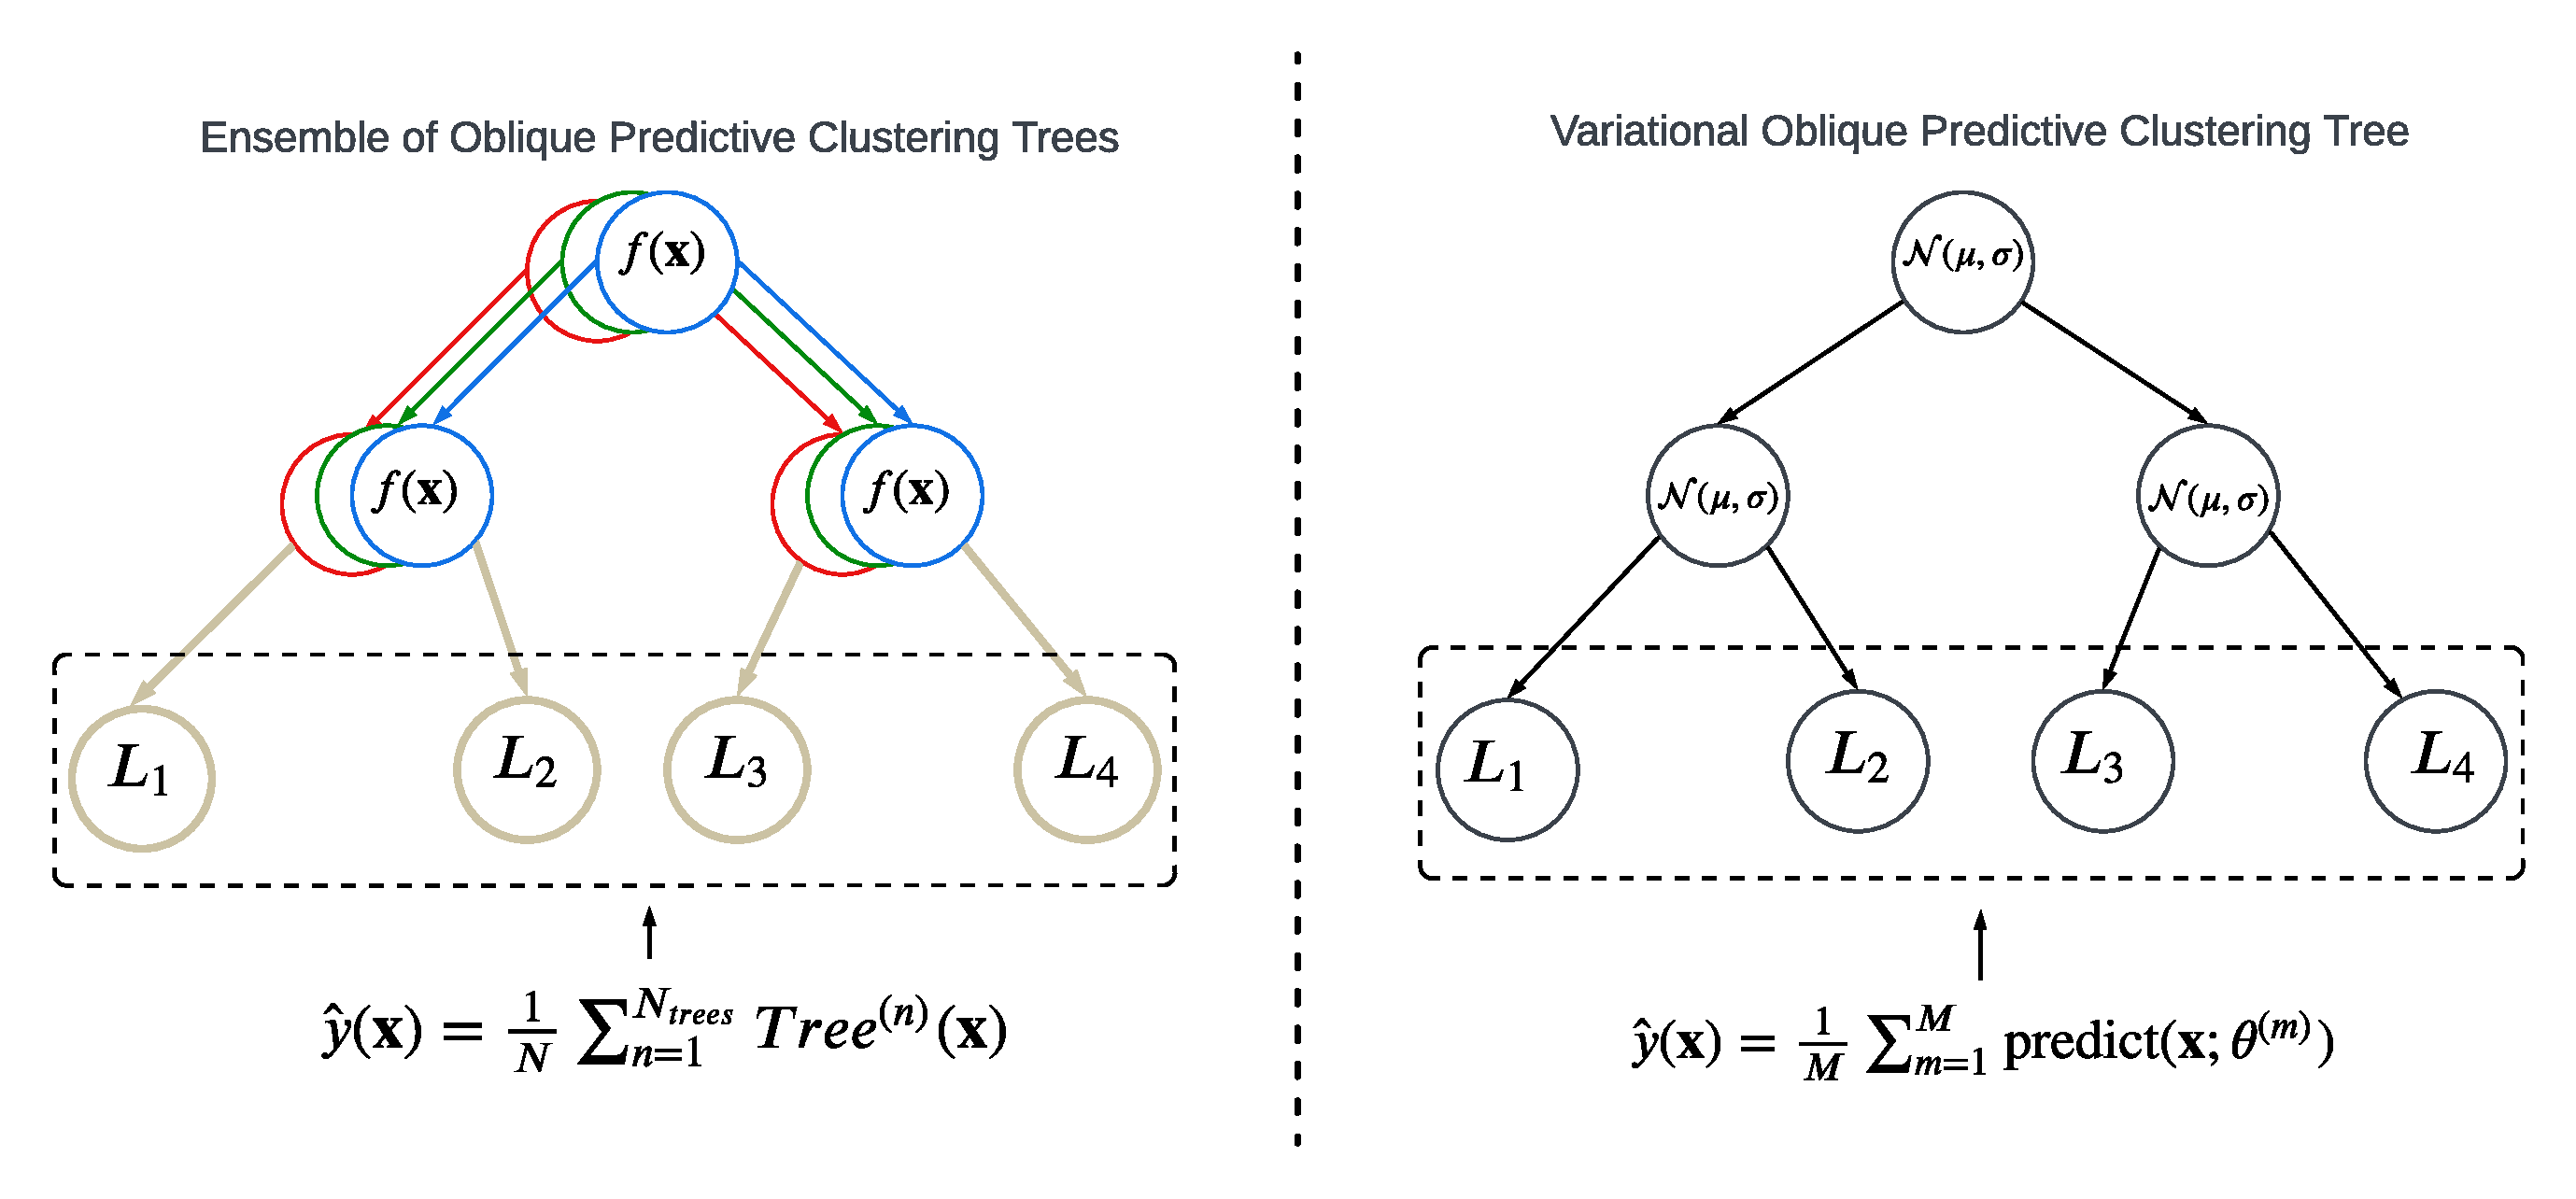
\includegraphics[width=1.0\textwidth]{main_flowchart.pdf}
    \caption{Ensemble of trees vs. Variational tree}
    \label{fig:main_flowchart}
\end{figure}

Our proposed \gls{vspyct} framework diverges from traditional ensemble approaches by directly incorporating Bayesian principles into oblique decision trees' architecture.
This model avoids conventional ensemble strategies, which aggregate multiple trees' outputs, for a probabilistic treatment of model parameters, offering refined mechanisms for uncertainty quantification and predictive performance.
The core of \gls{vspyct}'s innovation lies in applying the variational Bayes method for optimising parameters defining the oblique splits, and modelling these parameters as random variables with probability distributions.
This represents a paradigm shift toward a probabilistic understanding of decision-making processes within tree-based models, significantly enhancing interpretability, especially in uncertainty estimation domains.
It sets a new benchmark for interpretable, efficient, and reliable machine learning models.
\pbnote{Check Bayesian Additive Regression Trees (BART). Maybe add a comment/reference what is different}


%citiraj community detection (nasiot trud), rise of gen-ai/black-box ai/llms (llama, bert, gpt), post-hoc explainability (shap),  vb metodot, 

\section{Related work}

%references for VB applications in ML and Survival analysis models. Cite pavles paper.

\Glspl{pct} have been an essential development in extending decision tree capabilities to various predictive modelling tasks, including structured output prediction.
\Glspl{pct} are versatile and can be combined into ensembles to achieve state-of-the-art performance~\citep{Kocev_2013}.
However, as the dimensionality of the output space increases, the learning time of \glspl{pct} scales poorly, posing challenges in tasks like hierarchical multi-label classification where outputs can consist of hundreds of potential labels.

\Glspl{pct} are celebrated for their interpretability and efficiency, yet they often fall short in predictive performance due to their myopic, greedy selection of splits.
The introduction of option predictive clustering trees \pbnote*{use gls}{(OPCTs)}~\citep{Stepisnik_2020} aimed to address this limitation by incorporating multiple alternative splits within option nodes.
This approach mitigates the inherent myopia and achieves competitive performance with ensemble methods like bagging and random forests while still maintaining a degree of interpretability.
\pbnote*{use gls}{OPCTs}, despite mitigating myopia and enhancing performance, still face challenges in maintaining interpretability when extended to complex tasks.

On the other hand, \glspl{spyct}~\citep{Stepi_nik_2021} utilise oblique splits that incorporate linear combinations of features, allowing splits to correspond to arbitrary hyperplanes in the input space.
This makes \glspl{spyct} highly efficient for high-dimensional data and capable of leveraging data sparsity.
Experimental evaluations on numerous benchmark datasets have shown that \glspl{spyct} achieve performance on par with state-of-the-art methods while being significantly faster than standard \glspl{pct}~\citep{Andonovikj_2024}.
%Moreover, meaningful feature importance scores can be extracted from SPYCT models, enhancing their interpretability.

Despite these advancements, ensemble models such as random forests and gradient-boosting machines remain popular due to their superior predictive accuracy.
However, their complexity often obscures interpretability, making it challenging for users to understand the model’s decision-making process.
Efforts to bridge this gap include the iForest visual analytics system~\citep{Zhao_2019}, which summarises decision paths and tree structures within random forests, thereby making the ensemble's decisions more transparent.
Additionally, the Tree Space Prototypes approach~\citep{Tan_2020} uses representative points (prototypes) for each class, offering a more intuitive understanding of ensemble classifiers than traditional feature-based explanations.
Visual analytics systems like iForest and prototype-based approaches offer some clarity but do not fully resolve the complexity issue.

In critical applications, such as medical diagnosis, the need for transparent and trustworthy predictions is paramount.
Methods for explaining classifier predictions and estimating the reliability of regression predictions, as demonstrated in breast cancer recurrence prediction, provide users with additional insights and build trust by clarifying the decision-making process.
Similarly, the MAPLE~\citep{plumb2018model} model combines local linear modelling with a dual interpretation of random forests, offering faithful self-explanations and maintaining high predictive accuracy.
MAPLE addresses the accuracy-interpretability trade-off and provides both example-based and local explanations, making it a comprehensive tool for understanding model behaviour.
Methods like MAPLE and other interpretability frameworks strike a balance between accuracy and transparency, but they often fall short in handling high-dimensional, sparse data efficiently.

While significant progress has been made in improving decision tree models and their ensembles, several weaknesses remain.
Many of these approaches lack inherent mechanisms for uncertainty quantification, which is crucial for applications requiring high reliability and decision certainty.

Our proposed \gls{vspyct} model addresses these critical challenges by integrating Bayesian principles directly into the predictive clustering tree framework.
%Unlike traditional ensemble strategies, \glspl{vspyct} employs a probabilistic treatment of model parameters through the variational Bayes method, which enhances interpretability and provides inherent uncertainty quantification.
This approach maintains the clarity and simplicity of a single tree model while achieving state-of-the-art performance, thus offering a significant improvement over existing methods.
By introducing uncertainty quantification directly into the decision-making process, \gls{vspyct} enhances the reliability and applicability of the model across various domains where decision certainty is crucial.
%This advancement bridges the gap between theoretical developments and practical applications, marking a significant step forward in making complex decision trees more accessible, interpretable, and effective.


\section{The variational Bayes method}

% optional slika - Optimisation process of finding the closest variational distribution qω(θ) over the set of latent variables ω. (da se generira vo python)

In conducting a stochastic analysis, the process of inferring model parameters hinges on applying Bayes' theorem.
For observations $x$ produced by a system defined by parameters $\theta$, Bayes' theorem is given as:

\begin{equation}
p(\theta|x)=\frac{p(x|\theta)p(\theta)}{p(x)}
\label{eq:bayes_rule}
\end{equation}
The model-prescribed likelihood $p(x|\theta)$ and the selected prior $p(\theta)$ are generally well-defined.
The primary computational challenge arises in determining the posterior distribution $p(\theta|x)$ due to the denominator $p(x)$, which is derived as:

\begin{equation}
p(x)=\int_{\theta} p(x|\theta)p(\theta) \,dx,
\label{eq:evidence}
\end{equation}
This integral rarely yields a closed-form solution.
For cases with multiple dimensions, the computational burden often renders Monte Carlo methods infeasible.
The VB approach offers an approximation to this issue by closely mimicking the true posterior $p(\theta|x)$ with an approximate distribution $q_{\omega^*}(\theta)$. This variational distribution is part of a family of distributions $q_\omega(\theta)\in \mathcal{Q}$, parameterised by $\omega \in \Omega$, where $\Omega$ represents the potential latent parameter values.
Typically, the mean-field variational family is utilised, assuming independence among the parameters $\omega$~\citep{Blei_2017}. 
To find the optimal $\omega^*$, one minimises the \gls{kl} divergence $KL(q_\omega(\theta) \parallel p(\theta|x))$:

\begin{equation}
\omega^* = \argmin_{\omega \in \Omega}KL(q_\omega(\theta) \parallel p(\theta|x))
\label{eq:optim}
\end{equation}

Given the unknown nature of the true posterior, a rearrangement is needed to compute the \gls{kl} divergence, simplifying to~\citep[Chapter~10]{murphy2023probabilistic}:

\begin{equation}
KL(q_\omega(\theta) \parallel p(\theta|x)) = -\underbrace{\mathbb{E}_q\left[\log p(x,\theta) - \log q_\omega(\theta)\right]}_{\text{ELBO}}+ \log p(x)\\
\label{eq:kl_divergence}
\end{equation}

Maximising the \gls{elbo} serves to inversely minimise the \gls{kl} divergence between the approximate posterior \(q_\omega(\theta)\) and the true posterior \(p_\omega(\theta)\).
In the decomposition of the KL divergence, the term \(\log p(x)\), known as the marginal likelihood or evidence, remains constant with respect to the variational parameters \(\theta\).
Since this term does not involve \(\theta\), it does not influence the optimisation of the variational distribution and is thus excluded from the \gls{elbo} maximisation process.
By maximising the \gls{elbo}, we aim to tighten the bound provided by the \gls{kl} divergence, effectively making the variational posterior a better approximation of the true posterior.
Typically, the \gls{elbo} maximisation criterion is non-convex, with no assurance of global extremum convergence by optimisation algorithms~\citep[Chapter~10]{murphy2023probabilistic}.
Various algorithms have been proposed for this challenge, including variational EM \citep{bernardo2003variational}, stochastic variational inference~\citep{hoffman2013stochastic, sashank2018convergence}, amortised variational inference~\citep{gershman2014amortized, le2017inference}, and semi-amortised inference~\citep{kim2018semi}.

The adoption of an approximate variational distribution introduces bias contingent on the chosen variational family $\mathcal{Q}$, necessitating a decision grounded in empirical evidence or expert knowledge.
This bias arises because the family \(\mathcal{Q}\) may not be capable of capturing the true complexity of the posterior distribution~\(p_\omega(\theta)\).
As a result, the accuracy of the approximation depends significantly on how well \(\mathcal{Q}\) aligns with the true underlying distribution.
The choice of \(\mathcal{Q}\) thus not only affects the efficiency of the inference but also the quality and reliability of the model.
Despite this bias, VB's computational efficiency significantly surpasses traditional methods like Markov Chain Monte Carlo (MCMC).
In our case, the ADAM optimiser~\citep{kingma2014adam} is used to facilitate the \gls{elbo} optimisation.


\section{Methodology}

As the foundation of the \gls{vspyct} model, the underlying architecture closely follows that of the \gls{spyct} model, particularly in its tree construction process.
Similar to \gls{spyct}, \gls{vspyct} constructs a decision tree with an oblique structure, where each split is defined by a linear combination of input features, rather than relying on single-feature thresholds as in axis-aligned trees.

The key distinction between \gls{vspyct} and \gls{spyct} lies in the optimisation step used to determine the parameters of these oblique splits.
While \gls{spyct} utilises a deterministic approach to optimise split parameters, \gls{vspyct} introduces a probabilistic framework through variational Bayes (VB) optimisation.
\pbnote*{Maybe remove this whole part and merge it with the paragraph below since it repeats below~\eqref{eq:linear_model}.}{
In \gls{vspyct}, the parameters of the linear combination at each split—specifically, the weight vector \(\mathbf{w}\) and the bias term \(b\)—are modelled as random variables with Gaussian distributions.
This probabilistic representation of split parameters not only enhances the model's ability to handle uncertainty and noise in the data but also provides a measure of predictive uncertainty.
}

The construction of the \gls{vspyct} begins with a root node and proceeds iteratively, expanding the tree by adding internal nodes or leaf nodes in a manner identical to \gls{spyct}. Each node in the tree represents a binary decision point, where instances are split based on the oblique hyperplane defined by the linear model:

\begin{equation}
f(\mathbf{x}) = \sigma \left(\mathbf{w}^\top \mathbf{x} + b \right)
\label{eq:linear_model}
\end{equation}
where \(\mathbf{x} \in \mathbb{R}^N\) is the feature vector, \(\mathbf{w} \in \mathbb{R}^N\) represents the weight vector, \(b \in \mathbb{R}\) is the bias term, and \(\sigma(\cdot)\) denotes the sigmoid function, which ensures the output is a probability, determining whether an instance is sent to the right or left child node.

While the tree structure and the decision-making process follow the same principles as in \gls{spyct}, the optimisation of \(\mathbf{w}\) and \(b\) in \gls{vspyct} differs fundamentally.
In \gls{vspyct}, these parameters are not fixed but are instead inferred through variational Bayes optimisation.
The introduction of this probabilistic element distinguishes \gls{vspyct} from \gls{spyct}, enabling it to maintain the interpretability of a single decision tree while incorporating the robustness typically associated with ensemble methods.

\begin{comment}
\pbnote{Why noisy data, what if we have perfect data but wrong model}
\vanote{If we have perfect data - then even a deterministic model will do well for the prediction. We choose the type of model before we do the optimisation. If we choose a wrong model - e.g. a decision tree where it is simply a mismatch for the type of problem at hand - we will have bad predictive performance, regardless of the modelling framework (deterministic or probabilistic). But if we choose the right type of model, and face noisy data at test time - then a probabilistic model would capture the predictive uncertainty in its parameter distributions.}
\end{comment}


\subsection{Learning splits using Variational Bayes}

% optional: computation graph diagram

The goal is to update these prior distributions to approximate the posterior distributions given the observed data, thereby capturing the uncertainty in the model parameters.
The weights \(\mathbf{w}\) and bias \(b\) in the linear model, as in~\eqref{eq:linear_model}, are initially modelled with Gaussian prior distributions:

\begin{equation}
\mathbf{w} \sim \mathcal{N}(\mathbf{0}, \mathbf{I}), \quad b \sim \mathcal{N}(0, 1)
\end{equation}

The VB method aims to approximate the true posterior distributions of these parameters with a variational distribution \(q(\mathbf{w}, b|\mathcal{D})\).
We assume a simpler distributional form - a diagonal Gaussian:

\begin{equation}
q(\mathbf{w}, b|\mathcal{D}) = \mathcal{N}(\mathbf{w}|\boldsymbol{\mu}_w, \boldsymbol{\Sigma}_w) \mathcal{N}(b|\mu_b, \sigma_b^2),
\end{equation}
where \(\boldsymbol{\mu}_w\), \(\boldsymbol{\Sigma}_w\), \(\mu_b\), and \(\sigma_b^2\) are the parameters of the variational distribution, learned through the optimisation process.

The optimisation of the variational parameters is performed by maximising the \gls{elbo}, which serves as a lower bound to the log marginal likelihood \(\log p(\mathcal{D})\).
The \gls{elbo} is given by:

\begin{equation}
\mathcal{L}(\boldsymbol{\mu}, \boldsymbol{\Sigma}) = \mathbb{E}_{q(\mathbf{w}, b|\mathcal{D})}\left[\log p(\mathcal{D}|\mathbf{w}, b)\right] - KL\left(q(\mathbf{w}, b|\mathcal{D}) \parallel p(\mathbf{w}, b)\right)
\label{eq:elbo}
\end{equation}

The first term represents the expected log-likelihood of the data under the variational distribution, while the second term is the Kullback-Leibler (KL) divergence between the variational distribution and the prior. The \gls{elbo} is maximised using the ADAM optimiser, with the goal of refining the variational parameters \(\boldsymbol{\mu}\) and \(\boldsymbol{\Sigma}\) to closely approximate the true posterior.

The quality of a split is assessed using an impurity function, which is defined as:

\begin{equation}
\text{Impurity} = \sum_{i=1}^{N} \left(\rho_i \text{Var}_{\rho}(\mathbf{Y}) + \lambda_i  \text{Var}_{\lambda}(\mathbf{Y})\right),
\end{equation}
where \(\rho_i = \sigma(\mathbf{w}^\top \mathbf{x}_i + b)\) is the probability of an instance being routed to the right child node, and \(\lambda_i = 1 - \rho_i\) is the probability of routing to the left child node.
The variances \(\text{Var}_{\rho}(\mathbf{Y})\) and \(\text{Var}_{\lambda}(\mathbf{Y})\) represent the variance of the target variables in the right and left child nodes, respectively, weighted by their selection probabilities.
The objective is to minimise the impurity by optimising the parameters \(\mathbf{w}\) and \(b\) using the VB method, thereby ensuring that the split at each node effectively separates the data into homogeneous subsets.
The overall procedure for learning a split in \gls{vspyct} is detailed in Algorithm~\ref{alg:learn_split_vb}.
The algorithm involves initialising the variational parameters, performing Monte Carlo sampling to estimate the \gls{elbo}, and iteratively updating the parameters until convergence.

\begin{algorithm}[h!]
\caption{Variational Learning of Split Parameters in \gls{vspyct} with Impurity Minimization}
\label{alg:learn_split_vb}
\begin{algorithmic}[1]
    \State \textbf{Input:} $\mathcal{D} = \{\mathbf{X}, \mathbf{Y}\}$ (dataset), $\theta = \{\mathbf{w}_0, b_0\}$ (initial parameters), $E$ (epochs), $\lambda$ (learning rate), $\beta$ (batch size), $\sigma$ (selection probability)
    \State \textbf{Output:} $\Theta = \{\boldsymbol{\mu}_w, \boldsymbol{\Sigma}_w, \mu_b, \sigma_b^2\}$ (variational parameters)
 
    \Procedure{LearnSplit}{$\mathcal{D}, \theta, E, \lambda, \beta, \sigma$}
        \State Initialise $\Theta = \{\boldsymbol{\mu}_w, \boldsymbol{\Sigma}_w, \mu_b, \sigma_b^2\}$ \Comment{Initialise variational parameters}
        \State Initialise optimiser: $\alpha \gets \lambda$
        \For{$e \in \{1, \dots, E\}$} \Comment{Iterate over epochs}
            \For{each mini-batch $\mathcal{B} \subseteq \mathcal{D}$ of size $\beta$}
                \State Sample $\mathbf{w} \sim \mathcal{N}(\boldsymbol{\mu}_w, \boldsymbol{\Sigma}_w)$, $b \sim \mathcal{N}(\mu_b, \sigma_b^2)$
                \State Compute impurity $\Omega(\mathbf{X}, \mathbf{Y}; \mathbf{w}, b)$ as:
                \[
                \Omega(\mathbf{X}, \mathbf{Y}; \mathbf{w}, b) = \sum_{\text{right}} \rho(\mathbf{w}^\top \mathbf{x} + b) \cdot \text{Var}_\rho(\mathbf{Y}) + \sum_{\text{left}} (1 - \rho(\mathbf{w}^\top \mathbf{x} + b)) \cdot \text{Var}_\lambda(\mathbf{Y})
                \]
                \State Set the observed impurity value: $\Omega_\text{obs} = \frac{\Omega(\mathbf{X}, \mathbf{Y}; \mathbf{w}, b)}{2}$
                \State Condition on the observed impurity using:
                \[
                \log p(\Omega_\text{obs}|\Omega(\mathbf{X}, \mathbf{Y}; \mathbf{w}, b))
                \]
                \State Compute ELBO $\mathcal{L}(\mathcal{B}; \Theta)$ as per~\eqref{eq:elbo}
                \State Compute gradient $\nabla_{\Theta} \text{ELBO}$
                \State Update $\Theta \gets \Theta + \alpha \nabla_{\Theta} \text{ELBO}$ \Comment{Gradient descent update}
            \EndFor
            \If{early stopping criterion satisfied}
                \State \textbf{break}
            \EndIf
        \EndFor
        \State \textbf{return} $\Theta$
    \EndProcedure
\end{algorithmic}
\end{algorithm}



\subsection{Making a prediction}

The procedure for making a prediction for a new instance using the \gls{vspyct} model is detailed in Algorithm~\ref{alg:make_pred}.
The process involves traversing the tree from the root node to a leaf node, with decisions at each internal node being made \pbnote*{what do you mean by this? Are you referring to line 16 in algorithm 2?}{probabilistically} based on the parameters sampled from the learned variational posterior distributions.
The final prediction is determined by the prototype value stored in the reached leaf node.

Mathematically, at each internal node, the oblique split is determined by evaluating the linear combination of input features, with the parameters \(\Theta = (\mathbf{w}, b)\) drawn from their respective variational posterior distributions. The decision to branch left or right is based on the probability computed using the sigmoid function applied to this linear combination. This method accounts for the uncertainty in the model parameters, providing a probabilistic framework for decision-making.

The prediction \(\hat{y}\) returned by the model is the prototype of the reached leaf node, where the prototype is defined as the mean of the target values associated with the training instances that were routed to that leaf during training.

\begin{equation}
\hat{y} = \frac{1}{|\mathbf{Y}|} \sum_{i=1}^{|\mathbf{Y}|} y_i
\end{equation}
where \( y_i \) represents the target value of the \(i\)-th instance in \(\mathbf{Y}\).
This value $\hat{y}$ serves as the prediction for any new instance that reaches the particular leaf node.

\begin{algorithm}[h!]
\caption{Prediction Process in \gls{vspyct} using Monte Carlo Sampling}
\label{alg:make_pred}
\begin{algorithmic}[1]

\State \textbf{Input:} Feature vector $\mathbf{x}$, decision tree $T$ rooted at node $\Omega$, number of samples $M$
\State \textbf{Output:} Prediction $\hat{y}$

\Function{MC\_Predict}{$\Omega$, $\mathbf{x}$, $M$}
    \State Initialise $\hat{y}_{\text{sum}} = 0$
    \For{$m = 1$ to $M$}
        \State $\hat{y}_{\text{sum}} \gets \hat{y}_{\text{sum}} + \text{Predict}(\Omega, \mathbf{x}, m)$
    \EndFor
    \State \Return $\hat{y} = \frac{\hat{y}_{\text{sum}}}{M}$
\EndFunction

\Function{Predict}{$\Omega$, $\mathbf{x}$, $m$}
    \If{$\Omega$ is a leaf node}
        \State \Return $\hat{y}_\Omega = \frac{1}{|\mathcal{D}_\Omega|} \sum_{i \in \mathcal{D}_\Omega} y_i$
    \Else
        \State Sample $\Theta^{(m)} = (\mathbf{w}^{(m)}, b^{(m)})$ from $q(\mathbf{w}, b|\mathcal{D})$
        \State Compute $\rho(\Theta^{(m)}, \mathbf{x}) = \sigma(\mathbf{w}^{(m)\top} \mathbf{x} + b^{(m)})$
        \If{$\rho(\Theta^{(m)}, \mathbf{x}) \leq 0.5$}
            \State \Return \Call{Predict}{$\Omega_\text{left}$, $\mathbf{x}$, $m$}
        \Else
            \State \Return \Call{Predict}{$\Omega_\text{right}$, $\mathbf{x}$, $m$}
        \EndIf
    \EndIf
\EndFunction

\State \(\hat{y} \gets \) \Call{MC\_Predict}{$\Omega$, $\mathbf{x}$, $M$}
\State \textbf{Return} $\hat{y}$

\end{algorithmic}
\end{algorithm}

\subsection{Time complexity analysis}

We analyse the time complexity of learning a split in \gls{vspyct} and compare it with \gls{spyct}.
Our analysis focuses on the computational expense associated with determining a split, as this represents the principal distinction between the two approaches.
In the predictive clustering framework, the set of clustering attributes $K$, which contributes to the variance calculation, encompasses both the features and the target variables.
As a result, $K$ equals $D + T$, with $D$ representing the feature count and $T$ denoting the target count.
The time complexity for learning in \glspl{spyct} can be expressed as $\mathcal{O}(NI_o(D+K))$, wherein $N$ is the number of training instances, and $I_o$ is the iteration count needed for optimisation~\citep{Stepi_nik_2021}.
Notably, the computational demand for the \glspl{spyct}'s gradient-based version increases linearly with the attribute count.

The introduction of variational Bayes method in the architecture of the model adds a new layer of computational complexity.
Specifically, the complexity of learning a split in \gls{vspyct} is influenced by the following factors: the need to sample parameter sets from the approximative posterior distributions, the iterative optimisation required to refine these estimates towards minimising the \gls{elbo}, and the dimensionality imposed by the number of features.
The combined computational complexity for learning a split in \gls{vspyct} can thus be expressed as $\mathcal{O}(MNI_{vb}(D+K))$, where:
\begin{itemize}
\item $M$ represents the number of Monte Carlo samples needed to approximate the posterior distributions adequately.
\item $N$ is the number of data points evaluated during each iteration.
\item $D$ indicates the number of features, each contributing to the parameter space that must be sampled and optimised.
\item $K$ indicates the number of clustering attributes, used to calculate the variance in each of the node.
\item $I_{vb}$ indicates the number of iterations required for the variational inference process to achieve convergence.
\end{itemize}
This complexity reflects the multiplicative impact of sampling, feature dimensionality, and iterative optimisation, highlighting how the variational approach scales with the size and feature richness of the dataset.

Comparing \glspl{vspyct} to \glspl{spyct}, the VB method increases the computational load due to the necessity of Monte Carlo sampling and iterative \gls{elbo} optimisation.
However, this additional complexity is counterbalanced by the enhanced model interpretability, and uncertainty quantification offered by \glspl{vspyct}.

\subsection{Feature Importance}

The procedure for computing feature importance scores in \gls{vspyct} is inspired by the methodology introduced in the original \gls{spyct} model~\citep{Stepi_nik_2021}, while extending it to incorporate the model’s probabilistic nature.
Let \(\mathbb{E}[\mathbf{w}_s]\) and \(\text{Var}(\mathbf{w}_s)\) denote the element-wise mean and variance of the weights at node \(s\). We define:
\[
\mathbf{u}_s = \frac{\mathbb{E}[\mathbf{w}_s]}{\text{Var}(\mathbf{w}_s) + \epsilon}
\]
where \(\epsilon\) is a small constant added for numerical stability.
\pbnote{$\text{Var}(\mathbf{w}_s) > 0$, why do you need $\epsilon$? I know that we were talking about this, but there is a concept called coefficient of variation and it is defined as $\sigma/\mu$, std. (not variance) vs mean. We have to discuss this.}

The feature importance vector \(\text{Imp}(T)\) is then computed as:
\begin{equation}\label{eq:fimp}
\text{Imp}(T) = \sum_{s \in T} \left( \frac{s_n}{N} \right) \cdot \frac{|\mathbf{u}_s|}{\|\mathbf{u}_s\|_2}
\end{equation}
Here, \(\frac{s_n}{N}\) weights the contribution of node \(s\) by the fraction of training samples passing through it, and \(\|\mathbf{u}_s\|_2\) is the L2 norm of \(\mathbf{u}_s\).
This formulation integrates both the magnitude and the uncertainty of the weight parameters, potentially yielding a more robust measure of feature importance under a probabilistic model.
The vector $\mathbf{w}_s$ specifies the weights that define the oblique split at node $s$.
The expected value of the weights, $\mathbb{E}[\mathbf{w}_s]$, is computed through Monte Carlo simulation, where weights are sampled $M$ times from their approximation of the posterior distribution, and the mean of these samples is taken as the representative value for each weight.
This integrates the stochastic nature of the model parameters into the calculation of feature importance.
The repeated sampling and averaging process ensures that the estimated importance reflects both the central tendency and the variability of the weight parameters, crucial for interpreting the model's decision-making process under uncertainty.

\pbnote{For the toy example below, I would suggest to change the name from toy example to something else. Or completely remove the title.
Instead of using \emph{age} and \emph{salary} you can use $x_1$ and $x_2$.}
\paragraph{Toy Example}
Consider a simple dataset where two features, \textit{age} and \textit{salary}, predict the likelihood of purchasing a car.
In a \gls{vspyct} model, the influence of each feature at a node depends not only on the magnitude of its mean weight but also on how this mean compares to the feature’s weight variance.

Suppose that at the root node, the mean weights associated with \textit{age} and \textit{salary} are \( \mathbb{E}[w_{\text{age}}] = 0.2 \) and \( \mathbb{E}[w_{\text{salary}}] = 0.8 \), and their respective variances are \( \text{Var}(w_{\text{age}}) \) and \( \text{Var}(w_{\text{salary}}) \).
The importance at this node will now reflect the ratio \( \frac{\mathbb{E}[w]}{\text{Var}(w)} \), such that a feature with a relatively high mean weight but also a high variance will not necessarily dominate one with a slightly lower mean but substantially more \pbnote*{I don't know wheter the word stable is a correct one. May be precise because precission is the inverse of the variance.}{stable} (lower variance) weights.
Thus, if \textit{salary} maintains a higher \(\frac{\mathbb{E}[w]}{\text{Var}(w)}\) ratio than \textit{age}, it indicates that \textit{salary} is not only influential but also more reliably so at this particular node.

However, the overall feature importance is derived by aggregating these normalised ratios across all splits within the tree.
Even if \textit{salary} appears strongly influential at the root node, the final importance calculation considers both the magnitude and the stability of the weights across all nodes.
A feature consistently demonstrating a favourable \(\frac{\mathbb{E}[w]}{\text{Var}(w)}\) ratio throughout multiple splits will be deemed more important globally.
In this way, the final importance assessment accounts for both the strength and certainty of each feature’s contribution to the model’s decision-making process.


\section{Experimental setting}
\pbnote{The paragraph below is a little messy. I assume the idea is to say that we compare VBSPYCT on all benchmarks where OPCT and ensemble PCT were evaluated? If so write it like that.}
The experimental evaluation was conducted to compare the \gls{vspyct} model with several benchmarks, including the \gls{spyct} model, \glspl{opct}~\citep{Stepisnik_2020}, and ensemble of \glspl{pct}.
Specifically, we considered both a single \gls{spyct} and an ensemble of \glspl{spyct}, as well as a single \gls{opct} and an ensemble of \glspl{pct}.
We chose these methods as primary comparisons because they have been extensively evaluated in the literature, demonstrating strong performance across various \gls{sop} tasks~\citep{Andonovikj_2024, Stepi_nik_2021}.

The comparison encompassed a range of predictive modelling tasks, including single-target regression, multi-target regression, binary classification, and multi-class classification.
By evaluating not only a single \gls{spyct} tree, but also an ensemble of \glspl{spyct}, a single \gls{opct} tree, and an ensemble of \glspl{pct}, we aimed to assess how \gls{vspyct}'s predictive performance compares against a spectrum of models, from single decision trees to more complex ensembles and option-based trees.
This comprehensive approach allowed us to rigorously evaluate \gls{vspyct}'s effectiveness across different modelling scenarios and relative to both well-established baseline models and state-of-the-art tree-based methods.


\subsection{Data}

The experimental evaluation was performed on a diverse collection of datasets, each reflecting a distinct predictive modelling task: single-target regression (STR), multi-target regression (MTR), binary classification (BC), and multi-class classification (MCC).
The properties of these benchmark datasets are detailed in Tables~\ref{tab:str} through \ref{tab:mcc}, respectively.
Each table lists the number of examples (\(N\)) and the number of features (\(D\)) for all datasets, along with the number of targets (\(T\)) for MTR datasets and the number of classes (\(C\)) for MCC datasets.

\begin{table}[h!]
\centering
\caption{Properties of the benchmark STR datasets}
\label{tab:str}
\begin{tabular}{@{}lcccc@{}}
\toprule
\textbf{Dataset}   & \textbf{N} & \textbf{D} \\ \midrule
era~\citep{openml}                  & 1000         & 5          \\
cpmp~\citep{openml}                     & 2108         & 27          \\
qsar234~\citep{openml}                   & 2145         & 1026             \\
concrete\_compressive\_strength~\citep{openml}                   & 1030         & 9          \\
yprop~\citep{openml}                   & 8885         & 252       \\
puma8NH~\citep{openml}                & 8192         & 8        \\
spacega~\citep{openml}                  & 3107         & 6             \\
bike\_sharing~\citep{openml}           & 17379         & 6            \\
quake~\citep{openml}       & 2178         & 3         \\
ailerons~\citep{openml}         & 13750         & 40           \\ \bottomrule
\end{tabular}
\end{table}

\begin{table}[h!]
\centering
\caption{Properties of the benchmark MTR datasets}
\label{tab:mtr}
\begin{tabular}{@{}lccccc@{}}
\toprule
\textbf{Dataset}   & \textbf{N} & \textbf{D} & \textbf{T}     \\ \midrule
wq~\citep{openml}                  & 1060         & 16         & 14 \\
atp1d~\citep{openml}               &       337         & 411   &  6     \\
atp7d~\citep{openml}                   & 296         & 411       &  6    \\
scpf~\citep{openml}                   & 1137         & 23       &  3  \\
osales~\citep{openml}                   & 639         & 411   &  12  \\
sf1~\citep{openml}             &  323        & 10       &  3   \\
sf2~\citep{openml}                & 1066         & 10     & 3  \\
rf1~\citep{openml}                  & 9125         & 64       &  8    \\
rf2~\citep{openml}           &  9125        & 576       &  8   \\
slump~\citep{openml}       & 103         & 7   &  3    \\ \bottomrule
\end{tabular}
\end{table}

\begin{table}[h!]
\centering
\caption{Properties of the benchmark BC datasets}
\label{tab:str}
\begin{tabular}{@{}lcccc@{}}
\toprule
\textbf{Dataset}   & \textbf{N} & \textbf{D} \\ \midrule
scene~\citep{mulan}                  & 2407         & 299          \\
ova\_breast~\citep{openml}                     & 1545         & 10935          \\
ova\_lung~\citep{openml}                   & 1545         & 10935             \\
bio\_response~\citep{openml}                   & 3751         & 1777          \\
chronic\_kidney\_disease~\citep{openml}                   & 400         & 25       \\
compas\_two\_years~\citep{openml}             &  5278        & 13          \\
spambase~\citep{openml}                & 4601         & 57        \\
gina\_agnostic~\citep{openml}                  & 3468         & 970             \\
credit-g~\citep{openml}           & 1000         & 20            \\
diabetes\citep{openml}       & 768         & 8         \\ \bottomrule
\end{tabular}
\end{table}

\begin{table}[h!]
\centering
\caption{Properties of the benchmark MCC datasets}
\label{tab:mcc}
\begin{tabular}{@{}lccccc@{}}
\toprule
\textbf{Dataset}   & \textbf{N} & \textbf{D} & \textbf{C}     \\ \midrule
amazon\_reviews~\citep{openml}                  & 1500         & 10000   &  50     \\
dermatology~\citep{openml}                     & 366         & 34     &  6   \\
micro\_mass~\citep{openml}                   & 360         & 1300      &   10    \\
balance~\citep{openml}                   & 625         & 4       & 3  \\
yeast~\citep{mulan}                   & 1484         & 8    & 10  \\
wine~\citep{openml}             &  178        & 13     &  3   \\
mfeat\_zernike~\citep{openml}                & 2000         & 47   &  10   \\
har~\citep{openml}                  & 10299         & 561        &  6   \\
gas\_drift~\citep{openml}           & 13910         & 128      &   6   \\
semeion~\citep{openml}       & 1593         & 257    &   10  \\ \bottomrule
\end{tabular}
\end{table}

\mpop{In STR tasks, the output is a single continuous variable, while in MTR tasks, the output comprises multiple continuous target variables.
BC tasks involve two possible classes, and MCC tasks extend to multiple classes, with the exact number of classes depending on the specific dataset.
This comprehensive range of datasets ensures a robust evaluation of the models across varying complexity and output structures.}{}  


\subsection{Evaluation}

The performance of the models was evaluated using appropriate metrics for each predictive modelling task. For single-target regression, the Mean Absolute Error (\textit{MAE}) was employed as the evaluation metric:
\[
\textit{MAE} = \frac{1}{N} \sum_{i=1}^{N} \left| y_i - \hat{y}_i \right|
\]
where \( y_i \) denotes the true value, \(\hat{y}_i\) is the predicted value, and \(N\) is the total number of instances. A lower \textit{MAE} indicates better predictive accuracy.

For multi-target regression, a normalised Mean Absolute Error (\textit{NMAE}) was used to ensure comparability across targets with different value ranges. Letting \(y_{ij}\) and \(\hat{y}_{ij}\) be the true and predicted values for the \(j\)-th target of the \(i\)-th instance, and \(T\) be the total number of target variables, the \(\textit{NMAE}\) is defined as:
\[
\textit{NMAE} = \frac{1}{T} \sum_{j=1}^{T} \left( \frac{\frac{1}{N} \sum_{i=1}^{N} | y_{ij} - \hat{y}_{ij} |}{\max_i(y_{ij}) - \min_i(y_{ij})} \right)
\]
If \(\max_i(y_{ij}) - \min_i(y_{ij}) = 0\) for a given target \(j\), this denominator is replaced by 1, effectively leaving that target unscaled.

A lower \(\textit{NMAE}\) indicates better predictive performance, as it accounts for the range of each target variable to produce a comparable error measure across multiple targets.


For binary and multi-class classification tasks, the \textit{F1} score was used to measure model performance.
In the case of multi-class classification, the \textit{F1} score was macro-averaged across all classes.
A higher \textit{F1} score indicates better classification performance, as it reflects a balance between precision and recall.

All evaluations were conducted using 5-fold cross-validation, to ensure a comprehensive assessment of the model's performance across different subsets of the data, reducing the potential for bias and overfitting.


\section{Results}

Figure~\ref{fig:avg_rank} shows the average rankings of the evaluated methods \gls{vspyct}, \gls{opct}, single \gls{spyct}, ensemble of \glspl{spyct}, and ensemble of \glspl{pct} across four task types.
For improved readability, the actual performance of the models on each dataset is given in~\ref{app:res}.

\begin{figure}[h!]
    \centering
    \subfloat[BC]{%
        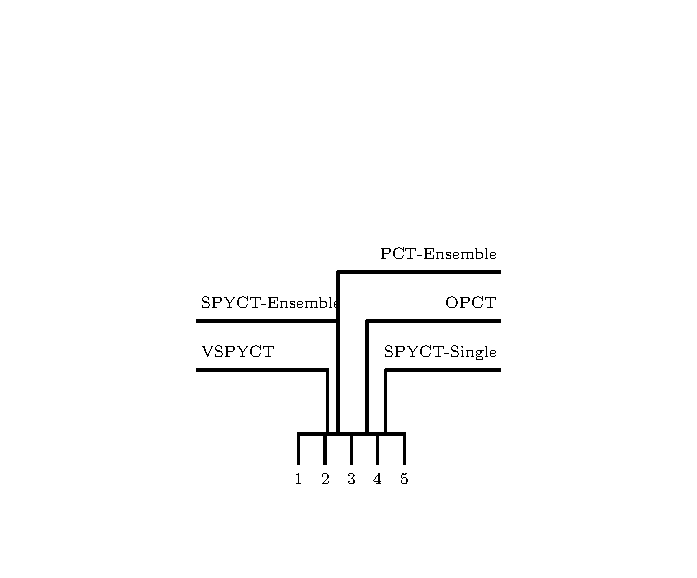
\includegraphics{critical_distance_bc.pdf}
        \label{fig:subfig1}
    }
    \subfloat[MCC]{%
        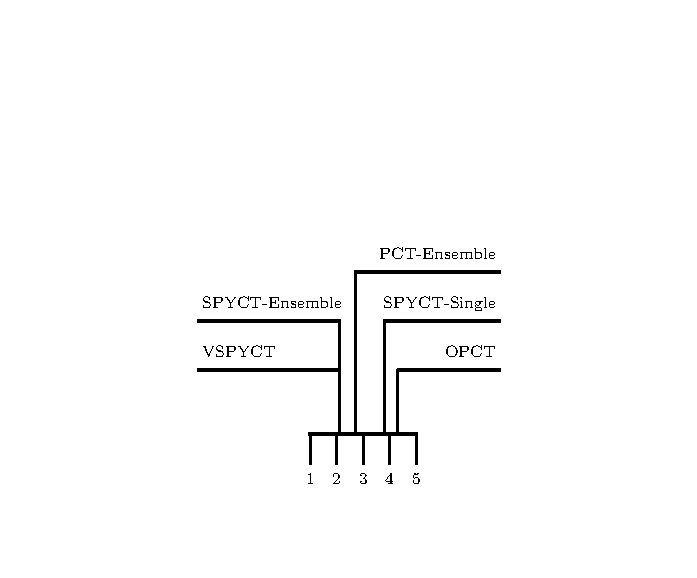
\includegraphics{critical_distance_mcc.pdf}
        \label{fig:subfig2}
    } \\
    \subfloat[STR]{%
        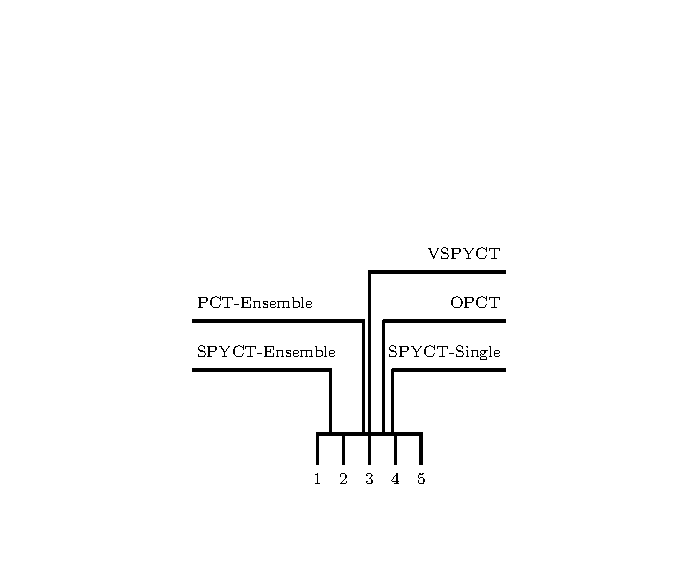
\includegraphics{critical_distance_str.pdf}
        \label{fig:subfig3}
    }
    \subfloat[MTR]{%
        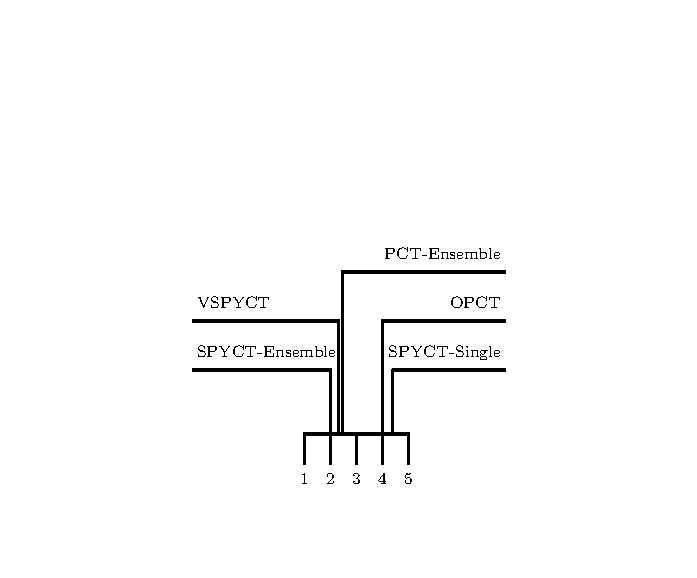
\includegraphics{critical_distance_mtr.pdf}
        \label{fig:subfig4}
    }
    \caption{Average rank of predictive performance. Lower ranks indicate better performance.}
    \label{fig:avg_rank}
\end{figure}

In BC tasks, \gls{vspyct} ranks first, outperforming ensembles of \glspl{spyct} and \glspl{pct}, which tie for second. This suggests that \gls{vspyct}’s probabilistic modeling effectively handles simple binary boundaries, surpassing both ensemble variance reduction and structural options (\gls{opct}).
In MCC tasks, \gls{vspyct} and the ensemble of \glspl{spyct} lead, followed by the ensemble of \glspl{pct}, single \gls{spyct}, and \gls{opct}, indicating that \gls{vspyct}’s uncertainty-aware splits can handle more complex class structures as well as ensembles can.

For STR tasks, both ensemble-based approaches—those combining multiple \glspl{spyct} and those combining multiple \glspl{pct}—achieve the highest ranks, followed by \gls{vspyct}.
It can be seen that ensembles appear particularly effective for precise single-target continuous predictions.
However, in MTR scenarios, \gls{vspyct} surpasses the ensemble of \glspl{pct}, indicating that its probabilistic representation of oblique splits can better capture complex inter-target relationships.
By contrast, \gls{opct} and single \gls{spyct} lag behind, indicating that their individual enhancements—option nodes or a single-tree oblique structure—do not offer sufficient complexity or flexibility to match the performance gains achieved by either ensembles or the probabilistic modelling of \gls{vspyct}.


\subsection{Discussion}

The results underscore the interplay between model complexity, uncertainty quantification, and variance reduction.
Ensemble methods consistently perform well in scenarios demanding high precision (e.g., STR) or broad generalisation over multiple outputs (MTR).
\Gls{vspyct}, capitalises on its Bayesian inference framework to excel in tasks where modeling uncertainty and complex decision boundaries are crucial (e.g., BC and MCC), and remains competitive even in more challenging regression contexts.

These findings underscore that \gls{vspyct} is not a universal replacement for ensembles, but rather a complementary alternative whose benefits depend on the task at hand.
When dealing with classification problems—binary or multi-class—where interpretability and uncertainty quantification are critical, \gls{vspyct} offers a potent blend of predictive performance, clarity, and inherent uncertainty modeling.
Its capability to handle intricate class boundaries and its flexibility in representing parameter uncertainties make it a valuable method for domains demanding transparency and robustness.

In continuous-output scenarios, ensembles still exhibit an edge, suggesting that if raw predictive precision is paramount and interpretability or uncertainty modeling are secondary considerations, ensemble models may remain the preferred choice.
Nevertheless, \gls{vspyct} provides a single-tree model that narrows the performance gap considerably and is particularly appealing when balancing predictive accuracy with the need for more direct insight into the model’s decision process.


\subsection{Feature importance scores}
\pbnote{Here you are missing some introduction why do you need this subsection.
Furthermore, when reading the complete subsection you have to clarify how did you add noisy features. What is the distribution of these features with respect to the original features?
Does this means that we have fearures that are completely useless in the original data, that even noise that does not influence the output is more important (since we have blue dots below the orange ones)?
One would expect only cases like in columns 2 and 3. 
}

\pbnote{
Just to be clear, originally you have this true model:
$$y=model(\mathcal{F}).$$
Based on this you fit one tree.
The you make
$$y_1=y+0\cdot\mathcal{F}'.$$
Now when I wrote it, it seems rather stupid notation.
Anyway, my question is how did you introduce this features.
Did you just add columns in the dataset with noise which in essence makes my model with $0\cdot\mathcal{F}'$ the correct explenation how you added the additional features?
}

\pbnote{
Is there a citation that can be used that discribes this way of thinking, how to evaluate feature importance metrics?
Or this is completely your idea?
}

\begin{figure}[h!]
    \centering
    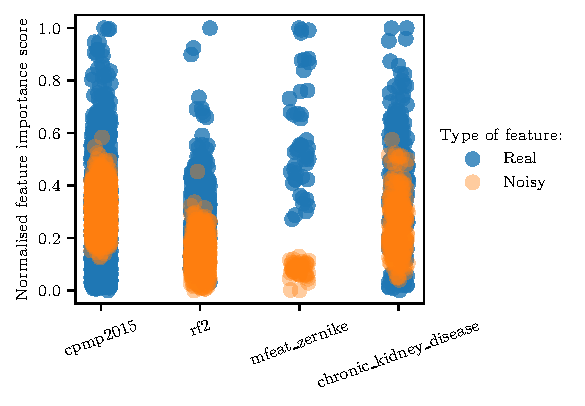
\includegraphics{../figures/feat_importances.pdf}
    \caption{Feature importance scores obtained on a single dataset from per category. The results indicate that the model does not depend on irrelevant features.}
    \label{fig:feature_importances}
\end{figure}

As illustrated in Figure~\ref{fig:feature_importances}, the proposed \gls{vspyct} model yields meaningful feature importance scores.
To rigorously evaluate this property, we introduced synthetic noise features into the datasets before model training.
Let the original dataset contain \(d\) features.
We then augmented it by adding \(d\) additional features, each generated by random noise.
Thus, the total number of features in the augmented dataset is \(2d\).

The resulting feature importance scores reveal that the original (real) features exhibit a broad range of importance values.
This heterogeneity is expected, as real-world datasets often comprise both highly informative variables and those with negligible predictive power.
In contrast, the artificially introduced noise features consistently received low importance scores.
Formally, if we let \(\mathcal{F} = \{f_1, f_2, \ldots, f_d\}\) denote the set of original features, and \(\mathcal{F}' = \{f_{d+1}, \ldots, f_{2d}\}\) the set of noise features, the estimated importances \(I(f_j)\) for \(f_j \in \mathcal{F}'\) are significantly lower than those for at least a subset of \(\mathcal{F}\).
This indicates that the \gls{vspyct}-derived importance measures are not only able to identify relevant features but also robust to the inclusion of spurious, non-informative features.


\subsection{Interpretability}

The dataset used for the interpretability analysis consists of $74,086$ anonymised instances of jobseekers from the Slovenian Public Employment Service (PES).
We will refer to it as the Unemployment dataset.
It includes a variety of personal and professional characteristics, such as age, gender, education, and work experience.
The target variable is the time until the jobseeker either becomes employed or exits the study, which is measured in days.
The dataset is challenging due to the different forms of its attributes (categorical, numerical, temporal) and the presence of censored data, where some jobseekers’ outcomes are not fully observed.

The goal is to predict the time-to-event (employment) for jobseekers, with some records being right-censored—meaning the exact time of the event is not observed.
Each data instance is described by features \(\mathbf{X}_i\), observed time \(t_i\), and a censoring indicator \(\delta_i\), where \(\delta_i = 1\) indicates the event was observed, and \(\delta_i = 0\) indicates a right-censored record.
This setup, with its inherent missing data due to censoring, makes it suitable for semi-supervised learning approaches.
Detailed information on the dataset and the semi-supervised multi-target regression framework can be found in~\cite{Andonovikj_2024}.

Figure~\ref{fig:pred_ci} presents the survival curve predicted by the \gls{vspyct} model for a specific jobseeker in the Unemployment dataset.
The curve shows the estimated probability of remaining unemployed over time, with the blue line representing the mean prediction.
The shaded area around the curve illustrates the uncertainty in the prediction, captured as a confidence interval between the 10th and 90th percentiles.
This visualisation effectively communicates the model's predictions along with its confidence, providing valuable insights into the jobseeker's likelihood of finding employment over time.
The dashed vertical line marks the actual observed time of employment, allowing for an immediate comparison between the predicted and actual outcomes.

\begin{figure}[h!]
    \centering
    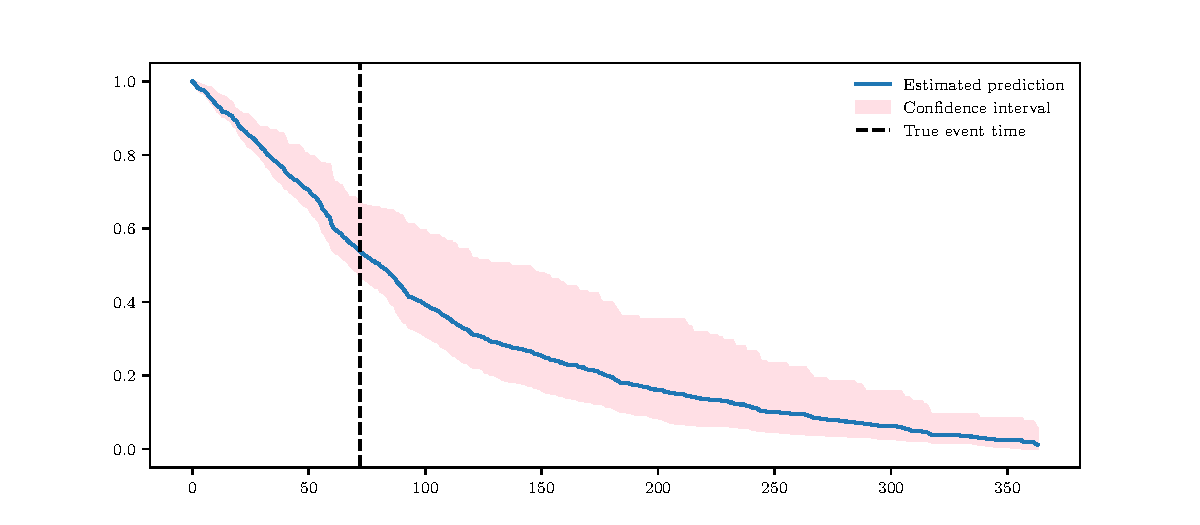
\includegraphics[width=1.0\textwidth]{pred_with_ci.pdf}
    \caption{Survival curve predicted by the \gls{vspyct} model on the Unemployment dataset. The blue line represents the estimated mean survival time, while the shaded area indicates the confidence interval (10th to 90th percentile) around the prediction. The vertical dashed line marks the actual time of the observed event.}
    \label{fig:pred_ci}
\end{figure}

Figure~\ref{fig:feature_importance} highlights the feature importance scores obtained from the \gls{vspyct} model, focusing on the most influential features that contribute to predicting the unemployment duration.
The horizontal bars show the relative importance of each feature, with \textit{Months of work experience} emerging as the most critical factor, followed by \textit{Age} and \textit{Entry month}.

\begin{figure}[h!]
    \centering
    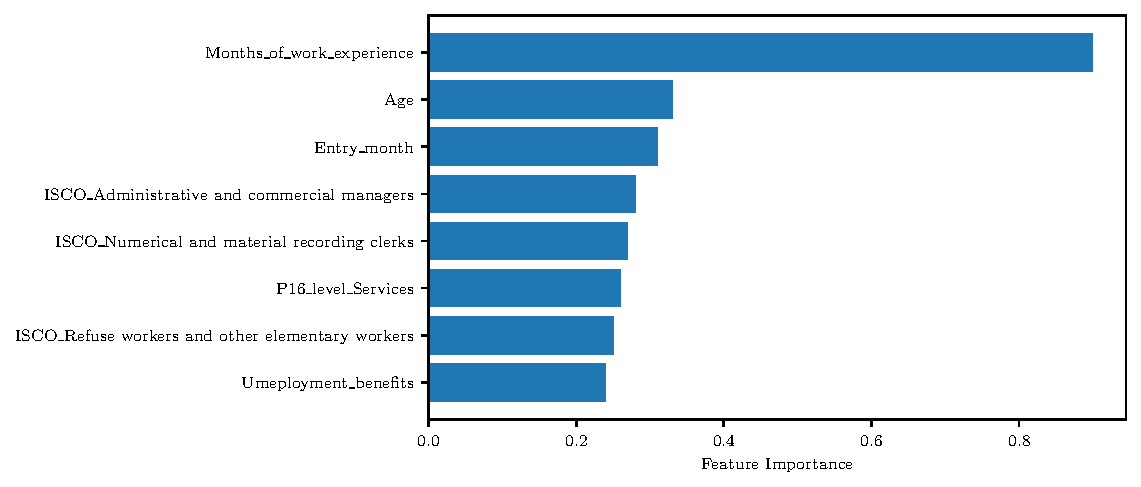
\includegraphics[width=1.0\textwidth]{feature_importance.pdf}
    \caption{Feature importance scores extracted from the \gls{vspyct} model applied to the Unemployment dataset. The horizontal bars represent the relative importance of each feature, with the most influential feature being "Months of work experience."}
    \label{fig:feature_importance}
\end{figure}

\begin{figure}[h!]
    \centering
    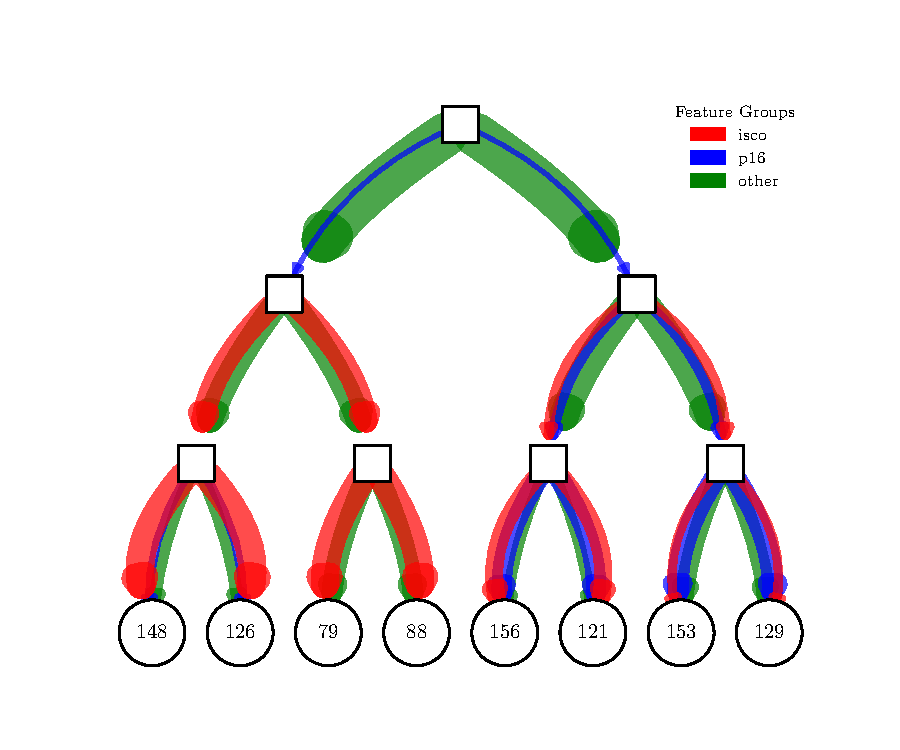
\includegraphics{hecat_tree_old_temp.pdf}
    \caption{The \gls{vspyct} model applied to the Unemployment dataset. The colouring distinguishes the different feature groups of the data set}
    \label{fig:inter_tree}
\end{figure}

Figure~\ref{fig:inter_tree} presents the visual representation of the \gls{vspyct} applied to the Unemployment dataset.
Based on that, one can distill a concise interpretation enriched with practical insights.

At the heart of this \gls{vspyct} model lies the ability to visually demarcate the influence of various feature categories on unemployment duration predictions.
The tree's root node is predominantly influenced by features categorised under ``other" (represented in green), encompassing age, months of work experience, and various demographic characteristics.
This indicates that such features play a pivotal role in initial split decisions, underscoring the broad impact of demographic and experiential factors on unemployment trends.

As we navigate through the tree, a dichotomy emerges based on the expected survival times—essentially, the projected duration an individual is likely to remain unemployed.
On branches leading to higher expected survival times, features categorised under ``p16 level of education" (coloured in blue) become increasingly dominant.
This suggests that higher levels of education are associated with longer periods of unemployment, potentially reflecting challenges in finding employment that matches an individual's qualifications or aspirations.

Conversely, on branches associated with lower expected survival times, the dominance shifts towards features represented by the ``ISCO classification of professional occupation" (coloured in red).
This dominance implies that certain professional occupations, as defined by the ISCO classification, may expedite reemployment, possibly due to higher demand or greater flexibility in job roles within these sectors.

This visual breakdown not only highlights the model's interpretability but also offers tangible insights into how different factors—ranging from personal demographics and work experience to education and professional classifications—impact unemployment durations.
Such insights are invaluable for policymakers and stakeholders aiming to devise targeted interventions that address specific barriers to employment faced by diverse demographic groups.

In essence, the \gls{vspyct} model's tree structure, with its intuitive colour-coded feature categories and quantified predictions at the leaf nodes, offers a powerful tool for understanding the multifaceted nature of unemployment.
It bridges the gap between complex machine learning models and practical socio-economic applications, providing a clear, actionable framework for addressing unemployment through informed, data-driven strategies.


\section{Conclusion}

We introduced the \gls{vspyct} model, an approach that combines the benefits of oblique splits, variational Bayes, and Bayesian inference within a single, interpretable predictive framework.
The \gls{vspyct} model addresses the trade-off between the performance of ensemble models and the interpretability of single decision trees, and the absence of inherent uncertainty quantification in predictions.
Our results demonstrate that the \gls{vspyct} model is competitive to, and on some datasets exceeds the performance of ensemble of \glspl{spyct}, without sacrificing the model's interpretability.
By employing variational Bayes method, we introduce a mechanism for uncertainty quantification directly into the decision-making process, enhancing the reliability and applicability of the model across various domains where decision certainty is paramount.
%The \gls{vspyct} model marks a significant step forward in making complex decision trees more accessible, interpretable, and effective.
The model opens new possibilities for research in semi-supervised learning and Bayesian inference, promising to bridge the gap between theoretical advancements and practical applications.
Future work will focus on further refining the model's performance, and extending its applications in diverse predictive tasks.

\begin{comment}
\section*{Acknowledgement}
The authors acknowledge the research core funding No.\ P2-0001,  P2-0103 and P2-0383 financially supported by the Slovenian Research Agency.
The authors also acknowledge the funding received from the European Union's Horizon 2020 research and innovation programme project HECAT under grant agreement No.\ 870702.
\end{comment}

%\printbibliography

\bibliographystyle{elsarticle-harv}
\bibliography{bibliography}

\appendix
\section{Detailed results}
\label{app:res}

\begin{table}[h!]
\centering
\caption{\textit{MAE} scores for STR (lowest is best)}
\label{tab:str_results}
\begin{tabular}{@{}lccccc@{}}
\toprule
Dataset & SPYCT-single & SPYCT-ensemble & VSPYCT & PCT-Ensemble & OPCT \\ \midrule
era                             & 1.296625 & \textbf{1.249352} & 1.287840 & 1.277622 & 1.277424 \\
cpmp2015                        & 384.377425 & 326.497515 & \textbf{285.105799} & 1211.124409 & 848.721320 \\
qsar234                         & 0.572577 & \textbf{0.415656} & 0.428724 & 0.428721 & 0.441020 \\
puma8NH                         & 2.795463 & \textbf{2.632242} & 2.711678 & - & - \\
yprop                           & 0.020126 & 0.019693 & 0.019969 & \textbf{0.019682} & 0.023687 \\
space\_ga                       & 0.105716 & 0.090193 & 0.104501 & \textbf{0.084793} & 0.099387 \\
bike\_sharing                   & 7.866288 & 3.101784 & 11.288880 & 10.610927 & \textbf{2.509829} \\
quake                           & 0.144549 & 0.143972 & \textbf{0.143805} & 0.147743 & 0.172350 \\
concrete\_compressive\_strength & 4.500918 & \textbf{4.121670} & 7.740371 & 4.164038 & 4.216046 \\
ailerons                        & 0.000135 & \textbf{0.000124} & 0.000127 & 0.000133 & 0.000161 \\
\bottomrule
\end{tabular}
\end{table}


\begin{table}[h!]
\centering
\caption{\textit{NMAE} scores for MTR (lowest is best)}
\label{tab:regression_results}
\begin{tabular}{@{}lccccc@{}}
\toprule
Dataset & SPYCT-single & SPYCT-ensemble & VSPYCT & PCT-Ensemble & OPCT \\ \midrule
wq       & 0.184654 & \textbf{0.167491} & 0.183236 & 0.169793 & 0.175325 \\
atp7d    & 0.321386 & 0.157284 & 0.167780 & \textbf{0.147780} & 0.176141 \\
atp1d    & 0.229711 & \textbf{0.104547} & 0.125300 & 0.106302 & 0.115277 \\
scpf     & 0.031613 & 0.027816 & \textbf{0.027291} & 0.047811 & 0.052046 \\
osales   & 0.068986 & 0.064457 & \textbf{0.057865} & 0.060054 & 0.058278 \\
sf2      & 0.042276 & 0.038311 & \textbf{0.037199} & 0.039234 & 0.041858 \\
sf1      & 0.097729 & 0.095937 & \textbf{0.092266} & 0.108493 & 0.109708 \\
slump    & 0.182132 & \textbf{0.165759} & 0.239199 & 0.175965 & 0.243881 \\
rf1      & 0.197493 & 0.183436 & \textbf{0.166669} & 0.167392 & 0.168493 \\
rf2      & 0.212579 & \textbf{0.176247} & 0.193914 & 0.177062 & 0.194180 \\
\bottomrule
\end{tabular}
\end{table}



\begin{table}[h!]
\centering
\caption{\textit{F1} scores for BC (highest is best)}
\label{tab:classification_results}
\begin{tabular}{@{}lccccc@{}}
\toprule
Dataset & SPYCT-single & SPYCT-ensemble & VSPYCT & PCT-Ensemble & OPCT \\ \midrule
scene                  & 0.944059 & \textbf{0.986098} & 0.972439 & 0.882295 & 0.935982 \\
ova\_breast            & 0.928256 & 0.946192 & 0.959834 & \textbf{0.966468} & 0.956409 \\
bioresponse            & 0.729417 & 0.777438 & 0.768986 & \textbf{0.777509} & 0.753144 \\
ova\_lung              & 0.802281 & 0.905439 & \textbf{0.920463} & 0.886492 & 0.904865 \\
chronic\_kidney\_disease & 0.961777 & 0.991777 & \textbf{1.000000} & 0.997178 & 0.997178 \\
compas\_two\_years     & 0.645271 & 0.641390 & 0.652540 & \textbf{0.666824} & 0.615251 \\
spambase               & 0.903289 & \textbf{0.934069} & 0.926491 & 0.924987 & 0.912740 \\
gina\_agnostic         & 0.856799 & 0.885768 & 0.858579 & 0.909199 & \textbf{0.922184} \\
credit-g               & 0.632353 & 0.657097 & \textbf{0.681566} & 0.615338 & 0.547619 \\
diabetes               & 0.698525 & 0.739710 & 0.715029 & \textbf{0.778026} & 0.694843 \\
\bottomrule
\end{tabular}
\end{table}



\begin{table}[h!]
\centering
\caption{\textit{F1} scores for MCC (highest is best)}
\label{tab:mcc_results}
\begin{tabular}{@{}lccccc@{}}
\toprule
Dataset & SPYCT-single & SPYCT-ensemble & VSPYCT & PCT-Ensemble & OPCT \\ \midrule
amazon\_reviews & 0.143184 & 0.331889 & 0.172791 & \textbf{0.333139} & 0.293184 \\
dermatology      & 0.852633 & 0.978408 & \textbf{0.980117} & 0.893882 & 0.922443 \\
micro\_mass      & 0.845445 & 0.940100 & \textbf{0.954908} & 0.940397 & 0.905830 \\
balance          & 0.645499 & 0.618803 & \textbf{0.825152} & 0.595340 & 0.585561 \\
yeast            & 0.443345 & 0.535824 & 0.471005 & \textbf{0.575664} & 0.443048 \\
wine             & 0.975580 & 0.965350 & 0.966350 & \textbf{1.000000} & 0.945825 \\
mfeat\_zernike   & 0.786454 & \textbf{0.804786} & 0.792283 & 0.759459 & 0.693469 \\
har              & 0.969661 & 0.982193 & \textbf{0.984686} & 0.942095 & 0.942095 \\
gas\_drift        & 0.974804 & \textbf{0.993256} & 0.988948 & 0.988421 & 0.981730 \\
semeion          & 0.846045 & \textbf{0.923838} & 0.868518 & 0.897004 & 0.811956 \\
\bottomrule
\end{tabular}
\end{table}



\end{document}
